\section{Johdanto}

Tämä kandidaatintyö käsittelee menetelmiä, joilla silmän fiksaatioita
voidaan tunnistaa katseentunnistuslaitteiden keräämästä datasta. Katseentunnistuksen tarkoituksena on selvittää minne ihminen on katsomassa. On yleisesti hyväksyttyä \citep[s.33]{munn2008}, että ne alueet, joihin ihmisen katse on suuntautunut ovat alueita, jotka ovat jollakin tapaa tärkeitä tai kiinnostavia katsojalleen. 

Analysoitaessa katseentunnistuslaitteden keräämää dataa jaetaan kerätyt datapisteet usein joko fiksaatioiksi tai sakkadeiksi. \citep[s. 71]{salvucci2000} Fiksaatio voidaan määritellä tarkoittamaan aluetta, johon katse pysähtyy \citep[s. 71]{salvucci2000} ja jonka aikana tapahtuu kognitiivista prosessointia, joka mahdollistaa ``näkemisen''  ihmiselle. \citep[s. 881]{Blignaut2009}

Fiksaatoiden tunnistaminen on usein ensimmäinen vaihe katseentunnistuslaitteen keräämän datan analysointia ja sen tarkoituksena on helpottaa korkeamman tason analyysin tekemistä identifioimalla olennaiset osat datajoukosta yhdistämällä datapisteitä fiksaatioiksi ja seulomalla siitä pois sakkadit, eli nopeat siirtymät fiksaatioista toiseen. \citep[s. 18]{mould2012}

Katseentunnistuslaitteiden ja usein niiden mukana tulevien valmiiden katsedatan analysointiohjelmistojen käyttäminen tutkimuksessa on tehnyt helpoksi aliarvioida merkityksen, joka käytetyllä fiksaation tunnistusalgoritmilla on lopulliseen analyysiin datasta. \citep[s. 111]{shic2008}
Tämän työn tavoitteena onkin auttaa katseentunnistuksesta kerättyä dataa hyödyntävää tutkijaa ymmärtämään taustalla käytetyn fiksaatioiden tunnistusalgoritmin merkitystä vastaamalla seuraaviin kysymyksiin:
\begin{itemize}
	\item Miten fiksaatio määritellään?
	\item Millaisia menetelmiä silmän fiksaatioden tunnistamiseen on olemassa?
	\item Millä tavalla näitä menetelmiä voidaan luokitella?
	\item Mitä asioita tulee ottaa huomioon käytettävän menetelmän valinnassa?
	\item Kuinka fiksaatiodataa voidaan yhdistää videokuvaan ihmisen näkökentästä?
	\item Kuinka esitellyt fiksaationtunnistusmenetelmät vertautuvat kaupalliseen toteutukseen?
\end{itemize}

Työ on rajattu niin, että siinä ei tulla käsittelemään erilaisia menetelmiä, joilla katseentunnistuslaite voi kerätä datansa. Työssä ei myöskään tulla selvittämään syvällisesti minkälaisia sovelluksia silmän liikedatan käytölle on olemassa. Työssä tullaan yllä esitettyjen tutkimuskysymysten mukaisesti keskittymään fiksaationtunnistusalgoritmeihin sekä siihen kuinka fiksaatiodataa voidaan yhdistää videokuvaan ihmisen näkökentästä.

Tutkimuskysymysten ratkaisemiseksi tehtiin kirjallisuuskatsaus tutkimukseen, jota havaitsemisen, psykologian ja konenäön aloilla on tutkimuskysymyksiin liittyen tehty. Tämän lisäksi työ sisältää kokeellisen osuuden, jossa verrataan kirjallisuudesta löydettyjen algoritmeja kaupallisen katseentunnistuslaitteen mukana tulleen ohjelmiston tuottamaan fiksaatiodataan. Vertailemalla kirjallisuudesta löytyviä menetelmiä kaupalliseen toteutukseen selvitetään kuinka lähelle kaupallisen toteutuksen tuloksia kirjallisuudesta löytyvillä menetelmillä on mahdollista päästä sekä kuinka haastavaa menetelmiä on toteuttaa. Näin tutkijan on mahdollista evaluoida, missä tapauksissa oman implementaation toteuttaminen olisi järkevää.

Yllä esitetyt tutkimuskysymykset tukevat työn rakennetta niin, että ne tullaan ratkaisemaan siinä järjestyksessä kuin ne on esitetty. Johdannon jälkeisessä luvussa ``Silmän liikeanalyysin tutkimus''  esitellään ja selitetään terminologiaa, jota tutkimuksen aihepiiriin kuuluu sekä esitetään kuinka tietoa tutkimukseen on haettu. VARMAAN JOTAIN MUUTA KANSSA...

Tämän jälkeen kolmannessa luvussa ``Silmän liikeanalyysin algoritmit''  esitellään kirjallisuudesta löytyneitä algoritmeja ja vertaillaan niitä toisiinsa kirjallisuuden perusteella. Tämän lisäksi luvussa esitellään taksonomia, jonka perusteella algoritmeja voi luokitella. Luvun perusteella lukija saa käsityksen siitä millaisia liikeanalyysin algoritmit tyyppillisesti ovat ja mitkä ovat kunkin esitellyn algoritmin vahvuudet ja heikkoudet.

Luvussa neljä ``Fiksaatioiden tunnistaminen liikedatasta''  sovelletaan kirjallisuudesta löydettyjä algoritmeja käytäntöön ja verrataan niiden tuloksia kaupallisen toteutuksen tuottamaan dataan. LISÄÄ TARVITAAN

Lopuksi johtopäätöksissä...
 

---------------------------------------------------------------
\section{Silmän liikeanalyysin tutkimus}

\section{Silmän liikeanalyysin algoritmit}
\subsection{Yksinkertainen nopeusraja-arvoon perustuva tunnistusalgoritmi I-VT}
I-VT fiksaationtunnistusalgoritmi on kaikista kirjallisuudesta esiin tulleista algoritmeista yksinkertaisin ja helpoin ymmärtää. Algoritmin ideana on, että lasketaan jokaisen datapistevälin nopeus ja pidetään pistevälejä joiden nopeus on pienempi kuin asetettu nopeusraja-arvo fiksaatioina ja pistevälejä joiden nopeus on suurempi kuin raja-arvo sakkadeina. Pistevälin nopeus on sama kuin pistevälin pisteiden etäisyys toisistaan, jos oletetaan, että datapisteiden välinen aika on vakio. Kun pistevälien nopeudet on laskettu, yhdistetään algoritmissa peräkkäiset fiksaatiopisteet fiksaatioryhmiksi ja hylätään sakkadipisteet. Lopuksi jokainen fiksaatioryhmä muutetaan muotoon <x,y,d,t>, jossa x:n ja y:n arvot lasketaan ryhmän keskiarvosta kummallekin muuttujalle. T:lle annetaan aika, joka kuului ensimmäiselle fiksaatioryhmään kuuluvalle pisteelle ja d:lle koko fiksaatioryhmän kesto. \citep[s. 73]{salvucci2000}

 Jotta I-VT algoritmia voisi käyttää tarvitsee sille määritellä vain yksi parametri, nopeusraja-arvo. Mikäli silmän etäisyys havainnoitavaan kohteeseen tunnetaan voidaan nopeusraja-arvo johtaa kulmanopeudesta, joka silmällä on suhteessa katsottavaan kohteeseen. Esimerkiksi \citet[s. 1099]{itti2005} on käyttänyt kulmanopeuden raja-arvona 20 astetta / sekunti niin kuin myös \citet[s. 73]{salvucci2000}:n mukaan \citep[s. 103-111]{megaw1984}.
Mikäli etäisyyttä havainnoitavaan kohteeseen ei tunneta niin nopeusraja-arvon määrittämisessä on vain käytettävä eksploratiivista data analyysia aineistoon, jossa otetaan huomioon mm. näytteenottotaajuus.

I-VT on yksinkertainen implementoida kuten liitteestä \emph{\nameref{sec:IVT-implementation}}  voidaan nähdä. Koska algoritmi käsittelee vain pientä osaa datajoukosta kerralla on se erittäin tehokas ja soveltuu hyvin reaaliaikaiseen datan analysointiin. \citep[s. 76]{salvucci2000} Suurimmat ongelmat algoritmilla esiintyvät silloin kun pistevälien nopeudet ovat lähellä raja-arvoa. Tällöin syntyy herkästi paljon fiksaatioryhmiä, joissa on vain muutamia peräkkäisiä pisteitä, jolloin näyttää helposti siltä, että fiksaatiota on todellista enemmän. Tätä ongelmaa on kierretty esimerkiksi ryhmittämällä tarpeeksi lähellä toisiaan olevat fiksaatioita yhteen katsealueiksi. \citep[s. 329]{just1980} Toinen keino ongelman kiertämiseksi on vaatia sakkadeilta minimikestoa. \citep[s. 103-111]{megaw1984}

\subsection{Dispersioraja-arvoon perustuva tunnistusalgoritmi I-DT}
I-DT tunnistusalgoritmin perustana on havainto siitä, että koska fiksaatiopisteillä on matala nopeus, on niillä taipumus kasaantua lähelle toisiaan. Algoritmi kerää datajoukosta peräkkäisten datapisteiden ryhmiä, joiden dispersio on annettua raja-arvoa pienempi ja merkitsee ne fiksaatioiksi. Tämän lisäksi koska fiksaatiot ovat tyypillisesti kestoltaan yli 100ms mittaisia, asetetaan algoritmissa myös minimi kestoaika, joka fiksaation tulee täyttää tullakseen tunnistetuksi. \citep[s. 74]{salvucci2000}

Algoritmin toteutuksessa voidaan käyttää ns. liikkuvaa ikkunaa yli peräkkäisten datapisteiden, josta kokeillaan täyttääkö ikkuna annetun dispersioehdon. Ikkuna alkaa datajoukon alusta ja ylittää aluksi minimikestoa vastaavaan määrän datapisteitä. Jos ikkuna täyttää dispersioehdon on kyseisen ikkunan datajoukko osa fiksaatiota jolloin ikkunan oikeaa etureunaa siirretään datapiste kerrallaan eteenpäin kunnes dispersioehto ei enää täyty. Kun fiksaation oikea reuna löytyy tallennetaan fiksaatio sen hetkisen ikkunan datapisteiden massakeskipisteen kordinaatteihin, jonka lisäksi fiksaatiolle asetetaan aloitusaika ja kesto. Kun fiksaatio on löytynyt, siirretään ikkuna alkamaan tunnistettua fiksaatiota seuraavasta pisteestä. Mikäli ikkuna ei täytä dispersioehtoa siirretään koko ikkunaa piste kerrallaan eteenpäin kunnes dispersioehto täyttyy tai datapisteet loppuvat. \citep[s.26-27]{gale1984}

Dispersioehto voidaan määritellä algoritmissa monella eri tavalla. Helposti ensimmäisenä mieleen tuleva tapa olisi pitää ehtona sitä, että jokaisen pisteen tulee olla maksimissaan ehdon määräämän etäisyyden päässä toisistaan. Tämän tavan heikkoutena on kuitenkin se, että jokaista pistettä pitää verrata jokaiseen toiseen pisteeseen, jolloin operaatioita tulee \(O(n^2)\). \citep[s.111] {shic2008} Edellistä tapaa voidaan approksimoida nopeasti laskemalla yhteen pisteiden isoin horisontaalinen ja vertikaalinen etäisyys toisistaan D = [max(x) - min(x)] + [max(y) - min(y)] \citep[s. 74]{salvucci2000}, jolloin kun uutta pistettä lisätään fiksaatioon, tarvitsee sitä verrata vain x:n ja y:n ääriarvoja vastaan.

Kolmas keino dispersioehdon määrittämiseksi on massakeskipiste-etäisyys metodi, jossa vaaditaan, että M N:stä pisteestä tulee olla raja-arvo etäisyyden sisällä N pisteen massakeskipisteestä. Edellä mainitulle metodille löytyy myös variantti, jossa M N:stä pisteen etäisyyksien normaalijakauma massakeskipisteeseen on maksimissaan asetettu raja-arvo. Jos ehtojen implementaatiota halutaan yksinkertaistaa voidaan M asettaa N:ksi. \citep[s.111] {shic2008}

I-DT tarvitsee siis toimiakseen kahta parametria, dispersioraja-arvoa sekä fiksaation minimikestoa. Mikäli silmän etäisyys katsottavaan kohteeseen on tunnettu voidaan dispersioraja-arvona käyttää etäisyyttä, joka syntyy vastakkaiselle kateetille 0,5-1 asteen kulmasta silmästä kohteeseen. Minimikestoksi voidaan antaa jokin arvo 100ms ja 200ms väliltä. \citep[s. 74]{salvucci2000}

I-DT on hieman monimutkaisempi implementoida kuin I-VT kuten liitteestä \emph{\nameref{sec:IDT-implementation}} voidaan nähdä, mutta edelleen kuitenkin kohtuullisen yksinkertainen. Algoritmi toimii lineaarisessa ajassa, jotenka se soveltuu I-VT:n tavoin reaaliaikaiseen fiksaatioiden tunnistukseen. Koska algoritmissa käytetään minimikestoa fiksaatiolle ei se kärsi samalla tavalla huojunnasta fiksaation ja sakkadin välillä, niin kuin I-VT voi tehdä. Suurimpana heikkoutena I-DT:llä on vahvasti toisistaan riippuvat kaksi parametria. Esimerkiksi pienellä dispersioraja-arvolla ja suurella fiksaation minimiajalla ei välttämättä löydetä yhtään fiksaatiota. Parametrien riippuvuus toisistaan tarkoittaa sitä, että niiden asettamisessa on oltava erityisen huolellinen.


\subsection{Markovin piilomalliin perustuva tunnistusalgoritmi I-HMM}

Markovin piilomalli (Hidden Markov Model, HMM) on tilastollinen malli, jonka taustalla on Markovin prosessi, jonka parametreja ei tunneta. Markovin piilomallin tavoitteena on pyrkiä päättelemään eri tilojen väliset siirtymätodennäköisyydet havaittavien lopputulemien perusteella. Markovin piilomalleja on käytetty laajasti puheentunnistuksen sekä käsialantunnistuksen tutkimuksessa.\citep[s. 257-286]{rabiner1989tutorial}

Kun fiksaatioiden tunnistamiseen sovelletaan Markovin piilomallia voidaan tunnistamisen ongelma jakaa kaksitilaiseen malliin kuten kuvasta~\ref{fig:hmm_sample} voidaan nähdä. 

\begin{figure}[h]
    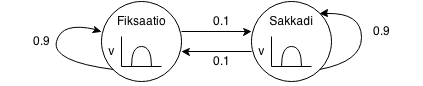
\includegraphics[width=1.0\textwidth]{HMM.png}
		\caption{Markovin piilomalli KORJAA JAKAUMAT!}
		\label{fig:hmm_sample}
\end{figure}

Malli koostuu havainto sekä siirtymätodennäköisyyksistä. Havaintotodennäköisyydet (v jakaumat kuvassa) edustavat tietyn tilan nopeuksien jakaumaa. Ensimmäinen tila edustaa fiksaatiota ja siitä johtuen sen nopeusjakauma on painottunut matalampiin nopeuksiin. Toinen tila edustaa sakkadeja ja vastaavasti sen nopeusjakauma on painottunut suurempiin nopeuksiin. Siirtymätodennäköisyyksiä esittävät kuvassa~\ref{fig:hmm_sample} esiintyvät nuolet ja ne tarkoittavat sitä todennäköisyyttä, jolla tila joko pysyy samana tai muuttuu sakkadista fiksaatioksi tai päinvastoin.

Malli tarvitsee toimiakseen kahdeksan parametria: molempien tilojen nopeusjakaumien keskiarvon ja varianssin sekä todennäköisyydet tilasiirtymille. Vaikka parametreja onkin enemmän kuin esimerkiksi nopeusraja-arvoalgoritmissa niin tämä ei ole ongelma, koska parametrien arvot ovat optimoitavissa harjoitteludatajoukon avulla menetelmällä nimeltä ``HMM uudelleen arviointi'' (HMM reestimation).\citep[s. 180]{salvucci1999} Suurin haaste tämän algoritmin käytössä onkin parametrien optimoinnin implementointi. Tähän olisikin suositeltavaa käyttää jotakin valmista kirjastoa, jos sellainen vain käytettälle ympäristölle on saatavissa.

Kun mallin parametrit on saatu määriteltyä voidaan mallia käyttää arvioimaan jokaiselle datajoukon pisteelle kuuluuko se fiksaatiohin vai sakkadeihin. Luokittelu tehdään HMM-dekoodaus menetelmällä, jossa etsitään todennäköisin sarja tiloja, joka määritellyn mallin perustella syntyy kun sille syötetään uusi datajoukko. Tämän todennäköisimmän sarjan laskentaan voidaan käyttää Viterbin algoritmia.\citep[s. 178]{salvucci1999}  Peräkkäiset fiksaatioiksi luokitellut pisteet yhdistetään myös toisiinsa samalla tavoin kuin nopeusraja-arvoalgoritmissa tehtiin.\citep[s. 31]{salvucci1999} Mallin parametrien optimoinnin jälkeen mallia voidaankin käyttää myös uusien datajoukkojen analysointiin, kunhan datajoukko on kerätty samassa ympäristössä ja olosuhteissa.

Markovin piilomalliin perustuva algoritmi toimii myöskin lineaarisessa ajassa kuten nopeusraja-arvo algoritmi, jotenka sitä voidaan käyttää myös reaaliaikaisuutta vaativissa ympäristöissä. Algoritmi tunnisti myös fiksaatiot tehokkaammin kuin nopeusraja-arvo algoritmi paljon häiriöitä sisältäneestä datasta \citet[s. 32]{salvucci1999}:n tekemässä tutkimuksessa.

\subsection{Pienimpään viritettyyn puuhun perustuva tunnistusalgoritmi I-MST}
I-MST-algoritmi on I-DT algoritmin ohella yksi tunnistusalgoritmeista, joka perustuu datapisteiden sijaintitiedon hyväksikäyttämiselle. Viritetyllä puulla tarkoitetaan puuta, joka kulkee graafin jokaisen pisteen kautta muodostamatta syklejä. Pienin viritetty puu on kaikista mahdollisista viritetyistä puista, joita graafista voidaan muodostaa se puu, jonka sivujen kustannusten muodostama summa on pienin. Sovellettaessa tunnistusalgoritmiin kustannuksella tarkoitetaan etäisyyttä, joka pistellä on toiseen pisteeseen.

Ensimmäiseksi algoritmissa jaetaan datajoukon pisteet osiin niin, että jokaisen osan pituus ajassa on se, mitä arvellaan pisimmän sakkadin datajoukossa olevan. Komogortsev käytti tutkimuksessaan tähän arvoa 200ms.\citep[s. 3 ]{komogortsev2010}. Tämän jälkeen jokaisesta osasta etsitään oma pienin viritetty puunsa. Graafi muodostetaan yhdistämällä jokainen osajoukon piste toisiinsa sivulla ja antamalla sivun kustannukseksi pisteiden välinen etäisyys. Pienimmän viritetyn puun löytämiseen voidaan käyttää Primin algoritmia.\citep[s. 75]{salvucci2000} Kun pienin viritetty puu on löydetty käydään sen pisteet läpi järjestyksessä jakaen pisteet sakkadeihin tai fiksaatiohin riippuen siitä onko etäisyys edelliseen pisteeseen suurempi vai pienempi kuin asetettu etäisyysraja-arvo.

On huomattava, että kun pienin viritetty puu muodostetaan ja fiksaatioita luokitellaan sen jälkeen, niin tietoa siitä missä järjestyksessä pisteet ovat alkuperäisessä datajoukossa ei oteta huomioon. Koska alkuperäinen datajoukko on alunperin jaettu pieniin osiin ennen puiden muodostamista, niin sillä että tieto puun pisteiden ajallisista suhteista hylätään ei ole juurikaan merkitystä. Itse asiassa tämä hylkääminen on algoritmille hyvä asia, koska silloin se kestää häiriöpisteitä hyvin. Esimerkiksi tilanteessa, jossa meillä on neljä peräkkäistä datapistettä, joista pisteet yksi, kaksi ja neljä ovat lähellä toisiaan ja kolmas piste on häiriöpiste kaukana muista, niin pisteet yksi, kaksi ja neljä tullaan luokittelemaan fiksaatioiksi, koska pisteistä muodostetussa pienimmässä viritetyssä puussa kolmas piste ei tule olemaan muiden pisteiden välissä vaan reunalla, jolloin ei muodostu kuin yksi sakkadiksi luokiteltava piste kahden sijasta, joka tapahtuisi jos käytettäisiin I-VT-algoritmia.

I-MST tarvitsee toimiakseen kaksi parametria: ajan jonka mukaan datajoukko jaetaan pienempiin osiin sekä etäisyysraja-arvon. Komogortsev ei tutkimuksessaan perustellut, mistä hänen käyttämänsä arvo 200ms datajoukon jakamiseen oli saatu muuten kuin, että se oli arvaus pisimmästä sakkadista, joka aineistossa esiintyisi. Parametrin asettamiseen ei siis ole automaattista tapaa vaan tutkija joutuu käyttämään jonkinlaista arvausta lähtökohtana. Etäisyysraja-arvon asettamiseen voitaneen käyttää samaa menetelmää kuin I-VT-algoritmissa vaikkakaan Komogortsev tai Salvucci eivät kumpikaan parametrin asettamista avaa tutkimuksissaan.

I-MST ei nopeudeltaan kilpaile muiden tässä työssä esiteltyjen algoritmien kanssa. Pienimmän viritetyn puun laskemisen kustannus kasvaa ekspotentiaalisesti, mitä enemmän pisteitä puuhun kuuluu. Eli toisin sanoen mitä suurempi näytteenottotaajuus datajoukossa on sitä raskaampaa I-MST-algoritmin käyttäminen on. 

Algoritmin implementointi on selvästi monimutkaisempaa kuin I-VT ja I-DT algoritmien, mutta yksinkertaisempaa kuin I-HMM-algoritmin. Mikäli algoritmia suunnittelee käyttävänsä on suositeltavaa käyttää jotakin kirjastoa, joka osaa laskea pienimmän viritetyn puun annetusta graafista. Tälläisia kirjastoja löytyy varmasti lähes jokaiselle ympäristölle, koska kyseessä on niin perustavanlaatuinen graafialgoritmi.

\subsection{Suorituskyvyn mittaaminen}
Jotta erilaisten fiksaationtunnistusalgoritmejen suorituskykyä olisi mahdollista verrata toisiinsa, on otettava käyttöön metriikoita, joilla tätä vertailua voidaan tehdä. Seuraavaksi esittelemme kirjallisuudesta löytyneitä menetelmiä vertailujen tekemiseen.

\citet[s. 4]{komogortsev2010} esittelee julkaisussaan erilaisia metriikoita fiksaationtunnistusalgoritmien vertailemiseen. Yksi näistä metriikoista on kvantitatiivinen fiksaatiopisteytys (engl. Fixation Quantitative Score FQnS). Metriikan käyttämiseen tarvitaan referenssijoukko datapisteitä, joista tiedetään esittävätkö pisteet fiksaatiota vai sakkadeja. Tälläinen datajoukko pitää käytännössä annotoida käsin tai vaihtoehtoisesti voidaan käyttää referenssinä katseentunnituslaitteen annotoimaa dataa niin kuin tässä työssä tullaan tekemään. Metriikan ideana on verrata algoritmin tunnistamien fiksaatioiden määrää referenssijoukossa olevien fiksaatioiden määrään.

\[
FQnS = 100 * {{tunnistetut fiksaatiot} \over {referenssifiksaatiot}}
\]
 
 Metriikan laskennassa käydään jokainen laskettavan datajoukon piste läpi ja mikäli piste on on arvioitu fiksaatioksi niin verrataan sitä vastaavan ajankohdan pisteeseen referenssijoukossa. Mikäli referenssijoukossa tuona ajankohtana oleva piste on fiksaatio niin kasvatetaan tunnistettujen fiksaatioiden määrää yhdellä. On huomattava, että FQnS:n laskennassa ei rangaista, mikäli referenssijoukon sakkadia luullaan fiksaatioksi. Näin ollen pelkästään tätä mittaria maksimoimalla ei saada hyvin toimivaa algoritmia, koska mittari voidaan maksimoida vain arvaamalla kaikki pisteet fiksaatioiksi.
 
 Toinen Komogortsevin julkaisussa esitetty metriikka on nimeltään kvalitatiivinen fiksaatioiden pisteytys (eng. Fixation Qualitative Score FQlS). Metriikkassa verrataan tunnistettuja fiksaatiopisteitä referenssidataan ja lasketaan keskimääräinen etäisyys, joka tunnistetulla fiksaatiolla ja referenssifiksaatiolla on toisistaan. 

\[
FQlS = {1 \over N} * \sum\limits_{i=1}^N etaisyys referenssifiksaatiosta_i
\]

metriikan nimeltä kvalitatiivinen fiksaatioiden pisteytys (eng. Fixation Qualitative Score FQlS). Metriikan käyttämiseen tarvitaan referenssijoukko datapisteitä, joista tiedetään esittävätkö pisteet fiksaatiota vai sakkadeja. Tälläinen datajoukko pitää käytännössä annotoida käsin tai vaihtoehtoisesti voidaan käyttää referenssinä katseentunnituslaitteen annotoimaa dataa niin kuin tässä työssä tullaan tekemään. 



\section{Fiksaatioiden tunnistaminen liikedatasta}

\label{sec:esimluku}

 --------------------------------------------------------------------

\section{Johtopäätökset}

Loppuluku päättää työn. Luvun nimi on tyypillisesti ``yhteenveto'' tai
``johtopäätöksiä''. Valitse se otsikko, joka tuntuu sopivammalta työsi
luonteeseen. Joka tapauksessa loppuluku sisältää niin työn yhteenvedon
kuin johtopäätöksiä työn tulosten perusteella. Pääajatus on antaa
lukijalle selvä kuva siitä, miten johdannossa asetettuihin
tavoitteisiin työssä vastattiin.

Käsittele loppupuvussa seuraavia asioita (jotakuinkin tässä järjestyksessä):
%
\begin{itemize}
  \item Muistutus työn tavoitteista (sidoksisuus johdantoon)
  \item Päätulokset kootaan yhteen, pohditaan niiden merkitystä
  \item Suositukset konkreettisiksi toimenpiteiksi (``Mitä sitten?'' 
Nyt kun käytössä on tämän työn myötä tullut tieto, 
mitä se nyt tarkoittaa tälle asialle/alalle.)
  \item Tulosten soveltuvuus, käyttöön liittyvät rajoitukset
  \item Jatkotutkimustarve 
(``Tulevaisuudessa olisi mielenkiintoista selvittää...'' tms.)
  \item Työn onnistumisen arviointi 
(Huom! Älä arvioi omaa kirjoitusprosessiasi vaan tekemääsi tutkimusta)
\end{itemize}

% --------------------------------------------------------------------

